\chapter{Objetivos}
\label{cap:capitulo2}

En esta sección del documento se describe el problema a resolver, marcando los los objetivos y requisitos pautados en el desarrollo del \ac{TFG}.

\section{Descripción del problema}
\label{sec:descripcion}

El objetivo principal de este \ac{TFG} es desarrollar un sistema de navegación autónoma capaz de realizar adelantamientos en entornos urbanos, empleando una combinación de aprendizaje por refuerzo con redes neuronales (\ac{DRL}) y diferentes técnicas de \ac{DL} para la percepción del entorno, con el fin de garantizar un comportamiento robusto, seguro y eficiente. El proyecto se centra en lograr una conducción suave y estable durante todo el recorrido, abordando tres subtareas principales: el seguimiento del carril para mantener la trayectoria correcta, el mantenimiento de una velocidad de crucero ajustada al vehículo delantero y la ejecución del adelantamiento, que incluye el cambio de carril y el retorno seguro al carril original.

A continuación, se definen los siguientes sub-objetivos: 

\begin{enumerate}
    \item Estudio del simulador CARLA \footnote{\url{https://carla.org/}}, con el objetivo de comprender sus capacidades y definir el entorno de desarrollo del \ac{TFG}, incluyendo la implementación de un sistema de teleoperación.
    \item Integración de sensores y técnicas de percepción, como la detección de carriles (con \textit{ground truth} y redes neuronales), segmentación semántica de imágenes captadas por la cámara y la división del \ac{LiDAR} en zonas de interés. Además, se desarrollará un sistema de seguimiento de carril basado en un controlador \ac{PID}.
    \item Desarrollo de comportamiento sigue-carril basado en algoritmos de \ac{DRL} para lograr una navegación 
    autónoma y eficaz.
    \item Expansión del sistema de control para incorporar comportamientos de velocidad de crucero y ejecución de adelantamientos.
    \item Análisis y comparación de los diferentes comportamientos desarrollados en el proyecto para validar su correcto funcionamiento.
\end{enumerate}

\section{Requisitos}
\label{sec:requisitos}

Los requisitos que han de cumplirse en este trabajo son: 
\begin{enumerate}
    \item Uso del entorno de simulación CARLA, que permite la creación de escenarios realistas y la emulación de diversos comportamientos de vehículos.
    \item Aprovechamiento de CARLA, un simulador ampliamente utilizado en el campo de la conducción autónoma, para probar modelos y garantizar la reutilización del proyecto en aplicaciones futuras relacionadas con la movilidad y la navegación autónoma.
    \item Integración de redes neuronales previamente desarrolladas para optimizar la percepción del entorno, mejorar la toma de decisiones del sistema autónomo.
    \item Comportamiento robusto y reactivo en tiempo real, asegurando una navegación segura y eficiente del vehículo en diferentes escenarios.
    \item Uso de los algoritmos \ac{DQN} y \ac{PPO} para el control autónomo del vehículo.
\end{enumerate}

\section{Metodología}
\label{sec:metodologia}

Este TFG comenzó en febrero de 2024 y finalizó en marzo de 2025. La metodología de trabajo fue la siguiente:

\begin{itemize}
    \item Reuniones semanales a través de \textit{Teams} \footnote{\url{https://www.microsoft.com/es-es/microsoft-teams/log-in}}, con una duración de entre 30 y 60 minutos, para hacer un seguimiento de los problemas que hubieran podido surgir durante la semana y definir los nuevos objetivos a cumplir.
    \item Contacto mediante el email de la universidad con el fin de solventar problemas urgentes e intercambiar contenido de avances significativos conseguidos.
    \item Se siguió la metodología tradicional \textit{Waterfall} \footnote{\url{https://asana.com/es/resources/waterfall-project-management-methodology}}, en la que el proyecto se desarrolló de manera secuencial, con cada fase dependiendo de la finalización de la anterior, garantizando un avance lineal desde el inicio hasta la finalización del proyecto.

	\begin{figure}[ht]
	  \begin{center}
	    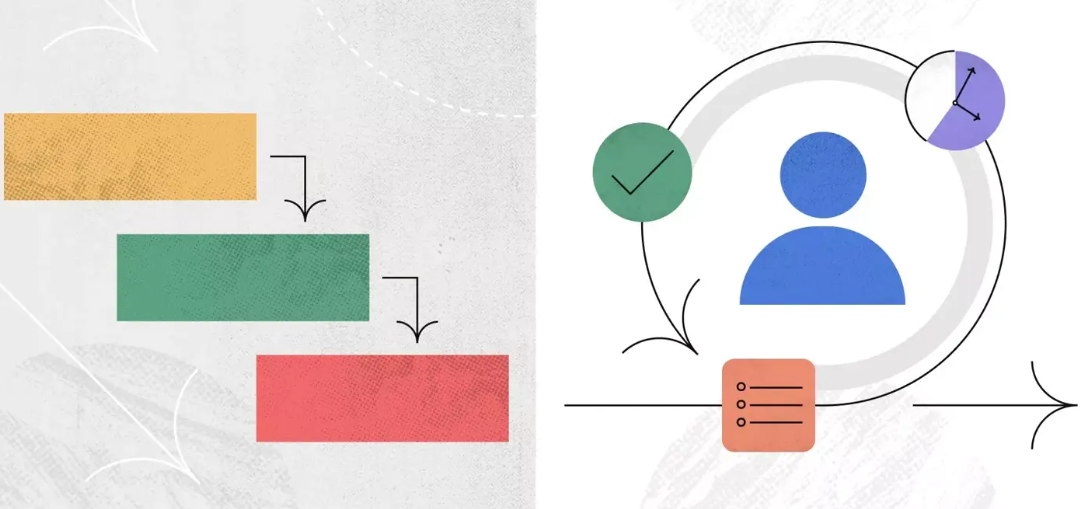
\includegraphics[width=7cm]{figs/objetivos/waterfall.png}
	  \end{center}
	  \caption{Metodología \textit{Waterfall}.}
	  \label{waterfall}
	\end{figure}

    \item Uso de un repositorio en \textit{GitHub}  \footnote{\url{https://github.com/}} para gestionar el control de versiones del código fuente, modelos y los datos más relevantes generados durante el desarrollo del proyecto.
    \item Mantenimiento de un \textit{blog} \footnote{\url{https://roboticslaburjc.github.io/2024-tfg-lara-poves/}} con el propósito de documentar problemas, avances e investigaciones realizadas durante la implementación del proyecto, asegurando un registro claro del progreso y soluciones de los desafíos superados.

	\begin{figure}[ht]
	  \begin{center}
	    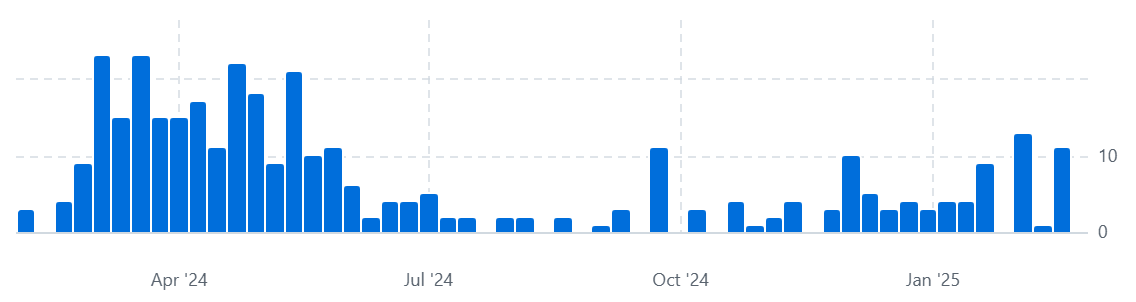
\includegraphics[width=9cm]{figs/objetivos/github.png}
	  \end{center}
	  \caption{Seguimiento de trabajo en GitHub.}
	  \label{github}
	\end{figure}

\end{itemize}

\clearpage

\section{Plan de trabajo}
\label{sec:plantrabajo}

Finalmente, los pasos a seguir de este trabajo han sido:

\begin{enumerate}
    \item Comienzo del trabajo:
	\begin{itemize}
		\item Desde el inicio, el tema del proyecto estuvo claro, centrado en la conducción autónoma en el simulador CARLA. El objetivo final sería lograr un comportamiento de adelantamiento mediante aprendizaje por refuerzo.
		\item Se gestionó el acceso al servidor donde se desarrollaría el proyecto, el cual ya contaba con el simulador instalado.	
		\item Se creó un entorno \textit{Conda} \footnote{\url{https://anaconda.org/}} y se procedió a la instalación de las librerías necesarias para el desarrollo.
	\end{itemize}

    \item Desarrollo del proyecto:
	\begin{itemize}
		\item Se desarrolló un teleoperador sencillo para explorar las diversas funcionalidades y configuraciones que ofrece el simulador CARLA.
		\item Se implementó el manejo de sensores como el \ac{LiDAR} y la cámara, los cuales se utilizarían posteriormente para lograr comportamientos específicos en el sistema autónomo. Además, se integraron redes neuronales para la detección de carriles y la segmentación semántica. Para la identificación del carril, se incluyó una nueva forma de deteccion basada en  \textit{ground truth} en CARLA.	
		\item Se configuró el autopiloto de CARLA, explorando las distintas opciones de configuración disponibles.
		\item Se desarrolló un sistema de seguimiento de carriles basado en un controlador \ac{PID}.
		\item En una primera etapa, se entrenó un modelo utilizando \ac{DQN} para que fuera capaz de seguir el carril. Posteriormente, se entrenó un nuevo modelo utilizando \ac{PPO} para mejorar el desempeño.
		\item Se realizó un reentrenamiento del último modelo para que pudiera mantener una velocidad de crucero utilizando la información proporcionada por el \ac{LiDAR} sobre el coche delantero.
		\item Finalmente, se reentrenó el modelo para extender el comportamiento y permitir la realización de adelantamientos en un entorno controlado.
	\end{itemize}

    \item Evaluación: Se compararon y analizaron los resultados obtenidos durante las diferentes fases y entrenamientos del proyecto.
    \item Se redactó la memoria del trabajo, documentando todo el proceso de investigación realizado.
\end{enumerate}

